\documentclass{standalone}
\usepackage[usenames,dvipsnames]{xcolor}
\usepackage{amsmath, amssymb, amsthm}

\usepackage{tikz}
\begin{document}
	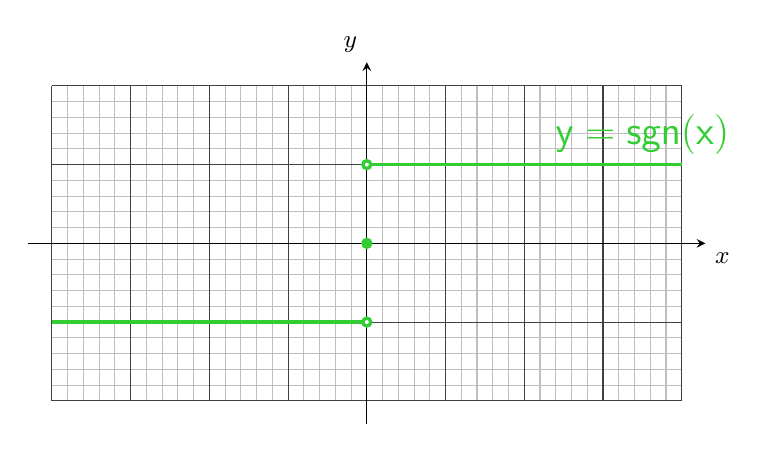
\begin{tikzpicture}[font=\small]
		\draw[black!25, step=0.2cm] (-4,-2) grid (4,2);
		\draw[black!75, step=1cm] (-4,-2) grid (4,2);
		\draw[black, -stealth] (-4.3,0) -- (4.3,0) node [below right] {$x$};
		\draw[black, -stealth] (0,-2.3) -- (0,2.3) node [above left] {$y$};
		\draw[very thick,color=LimeGreen] plot[domain=0:4] (\x, 1); 
		\draw[very thick,color=LimeGreen] plot[domain=-4:0] (\x, -1);
		\draw[very thick,color=LimeGreen, fill=LimeGreen] (0,0) circle (0.05cm); 
		\draw[very thick,color=LimeGreen, fill=white] (0,1) circle (0.05cm); 
		\draw[very thick,color=LimeGreen, fill=white] (0,-1) circle (0.05cm); 
		\draw[color=LimeGreen] (3.5,1) node [above] {\Large $\mathsf{y=\text{\textsf{sgn}}(x)}$};
	\end{tikzpicture}
\end{document}